\chapter{Appendices for Chapter \ref{Oliver_2026}}
\section{Deformations to the geostrophic contours}
\label{a:oddveven}
\subsection*{}
\noindent

We demonstrate that topography that is odd under the transformation \[\theta\rightarrow \pi - \theta\]
generates $O\lb \epsilon^{2}\rb $ variations to the geostrophic contours, while the harmonics that are even generate $O\lb \epsilon\rb $ variations. 
We restrict this analysis to geostrophic contours that form closed loops about the origin.
The following argument is general, but we will restrict the analysis to single harmonics, which is relevant to the present study. 
In this special case, we also obtain the leading order azimuthal dependence.

A symmetry property of the spherical harmonics is that
\[\hlm{\ell}{m}\lb \pi,\phi\rb = \lb -1\rb ^{\ell - m}\hlm{\ell}{m}\lb \pi-\theta,\phi\rb.\] 
We separately consider even and odd values of $\ell - m.$ The respective setups are illustrated in Figure \ref{f:sketch}.
\subsection*{$\ell - m$ is even}
Consider the geostrophic height function $H_{geo}$ associated with the boundary defined by equation (\ref{e:rcmb}) with $h\lb \theta,\phi\rb =\hlm{\ell}{m}$. 
Define $\hc\lb \theta,\phi\rb $ to be the extended chord which intersects the spherical surface $r=r_{o}$ at $\lb \theta,\phi\rb $ and $\lb \pi-\theta,\phi\rb.$  
Define $H_{\ell,m}^{\epsilon} = H_{\ell,m}^{\epsilon}\lb \theta,\phi\rb, $ to be the length of the portion of $\hc\lb \theta,\phi\rb $ which terminates at $r = \rcmb.$
The subscripts and superscript on $H_{\ell,m}^{\epsilon}$ indicate the structure and amplitude of the topography respectively. That is $H_{\ell,m}^{\epsilon} = H_{geo}$ for topography $\hLM$ with amplitude $\epsilon .$
We ignore regions near the poles (where the geostrophic cylinders extend from inner core to outer core) and the equator (where $H_{\ell,m}^{\epsilon}\rightarrow0$). 

$\hc$ intersects the surface $r = \rcmb$ at the polar angle $\theta_{1},$ which is slightly different than $\theta.$ There is not a closed expression for $\theta_{1},$ but
\[r_{o}\sin\theta = \ls r_{o} - \epsilon\hLM\lb \theta_{1},\phi\rb \rs\sin\theta_{1} \]
Assume that $\theta_{1}=\theta + \delta_{1},$ where $\delta_{1} \ll1.$
\[
	r_{o}\sin\theta \approx\ls r_{o}-\epsilon \hLM\lb \theta + \delta_{1},\phi\rb \rs \lb \sin \theta+\delta_{1} \cos\theta\rb 
\] 
Taylor expanding $\hLM$ and matching lowest order terms requires
\[\delta_{1} = \frac{\epsilon}{r_{o}}\hLM\lb \theta,\phi\rb \tan \theta \]
By the symmetry, $\hc\lb \theta,\phi\rb $ intersects the bottom hemisphere at the polar angle $\pi -\theta -\delta_{1}.$ Therefore
%
\[H_{\ell,m}^{\epsilon} = 2\cos \theta_{1}\ls r_{o} - \epsilon \hLM\lb \theta_{1},\phi\rb \rs \approx 2r_{o}\cos\theta -2\epsilon \hLM\lb \theta,\phi\rb \lb \cos\theta + \tan\theta \sin\theta\rb \]
%
\begin{equation}
	\implies H_{\ell,m}^{\epsilon}\approx 2r_{o}\cos\theta - \epsilon\; \lb \cos\theta + \tan\theta\sin\theta\rb \frac{1}{Q_{\ell}^{m}}P_{\ell}^{m}\lb \theta\rb\;  \cos m\phi.
	\label{e:hg_even}
\end{equation}
More succinctly, the leading order $\phi$ dependence of $H_{\ell,m}^{\epsilon}$ is $\cos m\phi$ at $O\lb \epsilon\rb .$ 

\subsection*{$\ell - m$ is odd}

The setup is the same as the previous section, except now $\hLM\lb \theta,\phi\rb = -\hLM\lb \pi-\theta,\phi\rb.$
We therefore consider the northern $\lb +\rb $ and southern $\lb -\rb $ hemispheres separately. 
In the previous section, the subscript $1$ was used to identify the polar angle $\theta_{1}$ at which $\mathcal{H}$ intersects the spherical boundary. 
The symmetry about the equator meant that we could use $\theta_{1}$ in both hemispheres.
We must now distinguish between the two, so we adopt a $+/-$ notation to refer to the upper ($+)$ and lower $(-)$ hemispheres. 
\[\delta_{\pm}\approx \pm\frac{\epsilon}{r_{o}}\hLM\lb \theta,\phi\rb \tan\theta \]
The geostrophic height is 
  \[H_{\ell,m}^{\epsilon}\lb \theta, \phi\rb = \ls r_{o}-\epsilon \hLM\lb \theta_{+},\phi\rb \rs \cos\theta_{+} +\ls r_{o}-\epsilon \hLM\lb \pi-\theta_{-},\phi\rb \rs \cos\theta_{-} \]
    \[
	    \begin{aligned}
		    \approx &\ls r_{o} - \epsilon \lb \hLM\lb \theta,\phi\rb  + \delta_{+} \frac{\partial \hLM}{\partial\theta}|_{\theta\phantom{\pi -}}\rb \rs \lb \cos \theta - \delta_{+}\sin\theta\rb \\
			    &\ls r_{o} + \epsilon \lb \hLM\lb \theta,\phi\rb  - \delta_{+} \frac{\partial \hLM}{\partial\theta}|_{\pi-\theta}\rb \rs \lb \cos \theta + \delta_{+}\sin \theta\rb
    \end{aligned}
    \]
     Expanding and collecting,
\begin{equation}
        H_{\ell,m}^{\epsilon} = 2 r_{o}\cos \theta + \epsilon \delta_{+}\ls 2\hLM \lb \theta,\phi\rb \sin\theta -  \cos\theta\lb\frac{\partial\hLM }{\partial\theta }|_{\theta\phantom{\pi-}} +\frac{\partial\hLM }{\partial\theta }|_{\pi-\theta}\rb\rs + O\lb \epsilon^{3}\rb
    	    \label{e:hodd}
\end{equation}

    The second term contains the leading order azimuthal dependence. Note that $\delta_{+}$ contains a factor of $\cos m\phi$. We can write the above approximation for $H_{\ell,m}^{\epsilon}$ as \[H_{\ell,m}^{\epsilon}\lb \theta,\phi\rb= 2 r_{o} \cos\theta + \epsilon^{2}\cos 2m\phi \;g\lb \theta\rb, \]
where $g$ is determined from equation ($\ref{e:hodd}$). 
The azimuthal order is doubled and the deformations are $O\lb \epsilon^{2}\rb. $ 
    


\begin{figure}
	\begin{center}
\subfloat[][]{
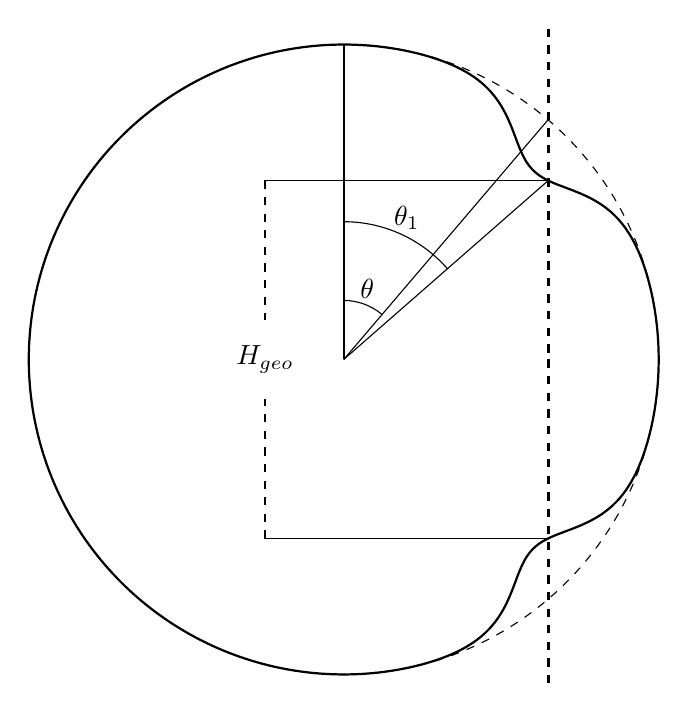
\begin{tikzpicture}

                \draw [color = black, dashed] (0,0) circle (4cm);
                \draw [color = black, thick,dashed] (2.6,4.2) --(2.6,0) ;
		\node at (2.9,3.5) {$\hc$};
		\draw [color = black, thick,dashed] (2.6,0) --(2.6,-4.2) node[left] {};
                \draw [color = black,thick] (0,0) --(0,4) node[left] {};
                \draw [color = black] (0,0) --(2.6,2.275) node[left] {};
                \draw [color = black] (0,0) --(2.6,3.05) node[left] {};
		\draw[color = black] (0,0.75) arc (90:50:0.75);
		\node at (0.3,0.9) {$\theta$};

		\draw[color = black] (0.00,1.75) arc (90:41:1.75);
		\node at (0.8,1.8) {$\theta_{1}$};
                \draw [color = black] (2.6,2.275) --(-1,2.275);
                \draw [color = black] (2.6,-2.275) --(-1,-2.275);
		\draw [color = black,dashed] (-1,-2.275)--(-1,-0.5);
		\draw [color = black,dashed] (-1,2.275)--(-1,0.5);
		\node at (-1,0) {$H_{geo} $};
        \draw [thick, color=black, domain=0:2*pi, samples=200, smooth]
	plot (xy polar cs:angle=\x r, radius={4-0.6*exp(-(\x-7*pi/4)^2/.05)-0.6*exp(-(\x-pi/4)^2/.05)});
\end{tikzpicture}
}
\quad
\subfloat[][]{
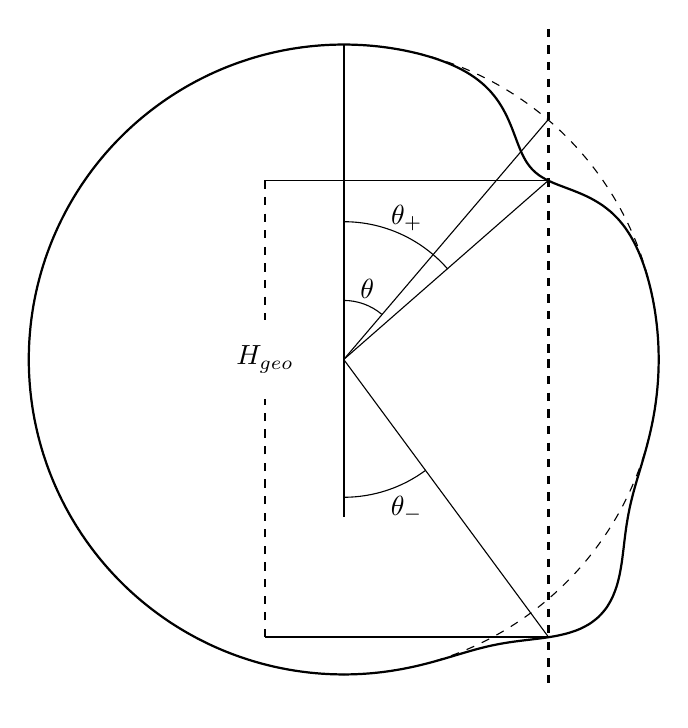
\begin{tikzpicture}

                \draw [color = black, dashed] (0,0) circle (4cm);
                \draw [color = black, thick,dashed] (2.6,4.2) --(2.6,0) ;
		\node at (2.9,3.5) {$\hc$};
		\draw [color = black, thick,dashed] (2.6,0) --(2.6,-4.2) node[left] {};
                \draw [color = black,thick] (0,-2) --(0,4) node[left] {};
                \draw [color = black] (0,0) --(2.6,2.275) node[left] {};
                \draw [color = black] (0,0) --(2.6,3.05) node[left] {};
		\draw[color = black] (0,0.75) arc (90:50:0.75);
		\node at (0.3,0.9) {$\theta$};

		\draw[color = black] (0.00,1.75) arc (90:41:1.75);
		\draw[color = black] (0.00,-1.75) arc (270:306.5:1.75);
		\node at (0.8,1.8) {$\theta_{+}$};
		\node at (0.8,-1.9) {$\theta_{-}$};
                \draw [color = black] (2.6,2.275) --(-1,2.275);
                \draw [color = black] (2.6,-3.525) --(-1,-3.525);
		\draw [color = black] (0,0)--(2.6,-3.525) ;
		\draw [color = black,dashed] (-1,-3.525)--(-1,-0.5);
		\draw [color = black,dashed] (-1,2.275)--(-1,0.5);
		\node at (-1,0) {$H_{geo} $};
        \draw [thick, color=black, domain=0:2*pi, samples=200, smooth]
	plot (xy polar cs:angle=\x r, radius={4+0.6*exp(-(\x-7*pi/4)^2/.05)-0.6*exp(-(\x-pi/4)^2/.05)});
\end{tikzpicture}
}
%\subfloat[][]{
%\begin{tikzpicture}
%
%                \draw [color = black, dashed] (0,0) circle (2cm);
%                \draw [color = black, thick,dashed] (1.3,1.1) --(1.3,0) node[left] {H};
%                \draw [color = black, thick,dashed] (1.3,0) --(1.3,-1.8);
%        \draw [thick, color=black, domain=0:2*pi, samples=200, smooth]
%	plot (xy polar cs:angle=\x r, radius={2+0.3*exp(-(\x-7*pi/4)^2/.05)-0.3*exp(-(\x-pi/4)^2/.05)});
%\end{tikzpicture}
%}
\end{center}
\caption[Geostrophic height function schematic]{(a) Topography that is even under the transformation $\theta\rightarrow \pi -\theta.$ (b) Topography that is odd.  $H_{geo}$ is the geostrophic height.}
\label{f:sketch}
\end{figure}

\section{Stability curves}
\label{a:bs_stab}
In this appendix we provide the values used to generate the stability curves presented in Figure \ref{f:bs_stab}. The curves are from the analysis of (BS96) \citep{pB96}, who use a different variable convention than presented in this study. For clarity, any variable with a star corresponds to the same variable, sans-star, in the BS96 paper.

The analysis adopts the Busse annulus, first proposed by Busse (1970) \citep{fB70}, which approximates a mid-latitude annular shell within the sphere. Sinusoidal, single wavelength, topography is imposed on the caps, extending along the rotation direction. 
We consider the mid-latitudes and use $\theta = 45^{\circ}$ (that is the slope parameter describing the annulus endcaps is $\eta^{*}=1$). 
The radial scale is chosen to be on the order of the bump wavelength, assumed to be much smaller than the vertical. That is
\[D^{*}= \frac{1}{m}\ll 2 r_o \cos\lb\theta\rb = 1.62.\]
We note that this requirement is only weakly met for $m = 4.$
The critical parameters in the theory are $\Gamma^{*} $ and $\mathcal{R}^{*},$ which can be related to $\epsilon$ and $Ra$ respectively by
 \[\Gamma^{*} =  Ek^{-1/4} \lb\frac{1}{D^{*}}\rb^{1/2}\epsilon\cos\lb\theta\rb \frac{m}{D^{*}},\]
 \[\mathcal{R}^{*} = Ra Ek \;2r_{0}\cos\lb\theta\rb\frac{\eta^{*}}{2}.\] 
For slow radial variation (that is $\beta^{*}=O\lb1\rb$ in the language of BS96), stationary convection (dotted lines in Figure \ref{f:bs_stab}) occurs above the curve drawn by 
\[\Gamma_{s}^{*} = \sqrt{\frac{m^{4} + m^{2} \mathcal{R}^{*^2}}{m^{2}\mathcal R^{*}}}.\]
Due to the quadratic dependency on $\mathcal{R}^{*},$ two values of $\mathcal{R}^{*}$ solve the above relation. The critical value is the lesser of the two, although both branches are shown in the Figure.
 At the smallest $\epsilon,$ the onset of convection is overstable (solid line in Figure \ref{f:bs_stab}), and occurs above the curve drawn by
 \[\Gamma_{s}^{*} = \sqrt{\frac{2 m^{2}}{\mathcal{R}^{*}}}.\]
 \section{Viscous torques}
 \label{a:visc_t}
\begin{figure}
	\begin{center}
		\includegraphics[width=0.5\textwidth]{Oliver_2026/figures/visc_topo_torque_ratio}
	\end{center}
	\caption[Viscous torques]{Ratio of the standard deviations of the viscous to topographic torques ($\gamma$) calculated at the CMB. We plot against topographic amplitude $\epsilon .$ Colors and markers correspond to the legend in Figure \ref{f:gs}. Values are less that  unity for all parameters except for the $\hlm{2}{1}$ topography at small $\epsilon$, which is associated with the smallest topographic torques. We expect $\gamma$ to decrease with $\Rat$ \citep{tO25}.}
	\label{f:viscrat}
\end{figure}
Previous work \citep[e.g.][]{bB07} has suggested that viscous torques do not play a large role in variations in LOD. In our previous study, we found that the ratio of viscous to topographic torques decreased as $\Rat$ increased. Therefore, viscous torques were not a major focus of the present work.
In Figure \ref{f:viscrat} we show $\gamma,$ the ratio of the standard deviations of the viscous to topographic torques. 
Except for the $\epsilon<0.1$, $\hlm{2}{1}$ topographies, where the topographic torques are very small, we find that $\gamma<1,$ indicating that topographic torques dominate over viscous torques. 
Roberts and Aurnou (2012) \citep{pR12} indicate that viscous torques should scales as $Re Ek^{-1/2}$ which is $O\lb 10^{6}\rb$ in our simulations and about the same size as our topographic torques. However in the core $Re Ek^{-1/2}$ is likely much smaller than $\Gstd \sim Re^{2}m_{c}\;\epsilon$.



\begin{table}
\begin{center}
\begin{tabular}{c c c c c c c c c c}
\hline
\hline
$\epsilon$ & Topography & $\Rat$ & $Ek$ & $\vartheta(r_{cmb})$ & $Re$ & $Re_w$ & $Re_{\gchar}$ & $Re_{\achar}$ & $Nu$\\
\hline
$0.0$ & -- & $40$ & $10^{-6}$ & 0 &$1278$ & $532.3$ & $936.1$ & $721.9$ & $6.1$ \\
 $0.01$ & $\hlm{2}{1}$ & $40$ & $10^{-6}$ & 0 &$1293$ & $540.9$ & $950.2$ & $729.0$ & $5.8$ \\
 $0.02$ & $\hlm{2}{1}$ & $40$ & $10^{-6}$ & 0 &$1293$ & $545.3$ & $946.9$ & $738.8$ & $5.8$ \\
 $0.05$ & $\hlm{2}{1}$ & $40$ & $10^{-6}$ & 0 &$1290$ & $545.2$ & $938.9$ & $728.0$ & $5.9$ \\
 $0.1$ & $\hlm{2}{1}$ & $40$ & $10^{-6}$ & 0 &$1298$ & $566.0$ & $910.9$ & $720.7$ & $6.1$ \\
 $0.2$ & $\hlm{2}{1}$ & $40$ & $10^{-6}$ & 0 &$1338$ & $602.6$ & $913.1$ & $710.5$ & $6.4$ \\
 $0.01$ & $\hlm{8}{4}$ & $40$ & $10^{-6}$ & 0 &$1303$ & $539.3$ & $964.7$ & $733.5$ & $5.8$ \\
 $0.02$ & $\hlm{8}{4}$ & $40$ & $10^{-6}$ & 0 &$1333$ & $545.4$ & $1006$ & $735.8$ & $5.9$ \\
 $0.05$ & $\hlm{8}{4}$ & $40$ & $10^{-6}$ & 0 &$1590$ & $567.2$ & $1257$ & $747.3$ & $6.2$ \\
 $0.1$ & $\hlm{8}{4}$ & $40$ & $10^{-6}$ & 0 &$1760$ & $558.8$ & $1503$ & $730.9$ & $6.4$ \\
 $0.2$ & $\hlm{8}{4}$ & $40$ & $10^{-6}$ & 0 &$2484$ & $726.9$ & $2156$ & $836.4$ & $10.0$ \\
 $0.01$ & $\hlm{32}{16}$ & $40$ & $10^{-6}$ & 0 &$1262$ & $547.6$ & $870.5$ & $725.6$ & $5.9$ \\
 $0.02$ & $\hlm{32}{16}$ & $40$ & $10^{-6}$ & 0 &$1304$ & $561.5$ & $879.1$ & $734.2$ & $6.1$ \\
 $0.05$ & $\hlm{32}{16}$ & $40$ & $10^{-6}$ & 0 &$1647$ & $616.5$ & $1339$ & $709.2$ & $7.0$ \\
 $0.1$ & $\hlm{32}{16}$ & $40$ & $10^{-6}$ & 0 &$1792$ & $739.8$ & $1448$ & $885.7$ & $9.0$ \\
 $0.2$ & $\hlm{32}{16}$ & $40$ & $10^{-6}$ & 0 &$2023$ & $811.8$ & $1657$ & $1091$ & $13.1$ \\
 $0.1$ & $\hlm{32}{17}$ & $40$ & $10^{-6}$ & 0 &$1679$ & $920.8$ & $957.9$ & $955.2$ & $10.3$ \\
 $0.01$ & $h_{t}$ & $40$ & $10^{-6}$ & 0 &$1305$ & $538.2$ & $942.4$ & $738.5$ & $6.1$ \\
 $0.02$ & $h_{t}$ & $40$ & $10^{-6}$ & 0 &$1288$ & $525.9$ & $934.0$ & $706.3$ & $6.4$ \\
 $0.05$ & $h_{t}$ & $40$ & $10^{-6}$ & 0 &$1309$ & $562.4$ & $929.5$ & $759.1$ & $6.4$ \\
 $0.1$ & $h_{t}$ & $40$ & $10^{-6}$ & 0 &$1379$ & $577.8$ & $958.1$ & $756.5$ & $6.8$ \\
 $0.2$ & $h_{t}$ & $40$ & $10^{-6}$ & 0 &$1510$ & $631.7$ & $1073$ & $781.2$ & $7.1$ \\
 \hline
 \hline
 \end{tabular}
\end{center}
\caption[Run parameters for turbulent simulations]{Run parameters for turbulent simulations. The aspect ratio is $\chi = 0.35$ and the Prandtl number is $Pr = 1$. Resolution was $230400$ elements each with $8^3$ grid points ($1.18\times10^{8}$ total points).}
\label{t:p_space}
\end{table}
\begin{table}
\begin{center}
\begin{tabular}{c c c c c c c c c c}
	\hline
\hline
$\epsilon$ & Topography & $\Rat$ & $Ek$ & $\vartheta(r_{cmb})$ & $Re$ & $Re_w$ & $Re_{\gchar}$ & $Re_{\achar}$ & $Nu$\\
\hline
$0.01$ & $\hlm{8}{4}$ & $0.01$ & $10^{-6}$ & 0&$*$ & $*$ & $*$ & $*$ & $*$ \\
 $0.01$ & $\hlm{8}{4}$ & $0.1$ & $10^{-6}$ & 0&$*$ & $*$ & $*$ & $*$ & $*$ \\
 $0.01$ & $\hlm{8}{4}$ & $1.0$ & $10^{-6}$ & 0&$13.0$ & $6.89\times 10^{-1}$ & $20.2$ & $1.53$ & $1.00$ \\
 $0.02$ & $\hlm{8}{4}$ & $0.01$ & $10^{-6}$ & 0&$*$ & $*$ & $*$ & $*$ & $*$ \\
 $0.02$ & $\hlm{8}{4}$ & $0.1$ & $10^{-6}$ & 0&$*$ & $*$ & $*$ & $*$ & $*$ \\
 $0.02$ & $\hlm{8}{4}$ & $1.0$ & $10^{-6}$ & 0&$37.6$ & $2.33$ & $34.1$ & $3.21$ & $1.03$ \\
 $0.05$ & $\hlm{8}{4}$ & $0.01$ & $10^{-6}$ & 0&$*$ & $*$ & $*$ & $*$ & $*$ \\
 $0.05$ & $\hlm{8}{4}$ & $0.1$ & $10^{-6}$ & 0&$10.2$ & $2.35\times 10^{-1}$ & $13.8$ & $4.38\times 10^{-1}$ & $1.02$ \\
 $0.05$ & $\hlm{8}{4}$ & $1.0$ & $10^{-6}$ & 0&$55.6$ & $4.06$ & $50.7$ & $5.70$ & $1.15$ \\
 $0.1$ & $\hlm{8}{4}$ & $0.01$ & $10^{-6}$ & 0&$4.52$ & $7.26\times 10^{-2}$ & $4.23$ & $7.97\times 10^{-2}$ & $1.04$ \\
 $0.1$ & $\hlm{8}{4}$ & $0.1$ & $10^{-6}$ & 0&$25.0$ & $7.56\times 10^{-1}$ & $23.2$ & $9.57\times 10^{-1}$ & $1.18$ \\
 $0.1$ & $\hlm{8}{4}$ & $1.0$ & $10^{-6}$ & 0&$87.9$ & $7.49$ & $82.1$ & $10.0$ & $1.43$ \\
 $0.2$ & $\hlm{8}{4}$ & $0.01$ & $10^{-6}$ & 0&$8.11$ & $4.02\times 10^{-1}$ & $7.58$ & $5.36\times 10^{-1}$ & $1.19$ \\
 $0.2$ & $\hlm{8}{4}$ & $0.1$ & $10^{-6}$ & 0&$37.6$ & $2.64$ & $34.4$ & $3.80$ & $1.48$ \\
 $0.2$ & $\hlm{8}{4}$ & $1.0$ & $10^{-6}$ & 0&$135$ & $18.7$ & $120$ & $29.9$ & $2.23$ \\
 \hline
 \hline
 \end{tabular}
\end{center}
\caption[Run parameters for subcritical simulations]{Run parameters for subcritical simulations.  Values denoted with a $*$ correspond to runs that were prohibitively expensive to saturate. The aspect ratio is $\chi = 0.35$ and the Prandtl number is $Pr = 1$. Resolution was $33600$ elements each with $8^3$ grid points ($1.72\times10^{7}$ total points).}
\label{t:p_space2}
\end{table}\begin{table}
\begin{center}
\begin{tabular}{c c c c c c c c c c}
	\hline
\hline
$\epsilon$ & Topography & $\Rat$ & $Ek$ & $\vartheta(r_{cmb})$ & $Re$ & $Re_w$ & $Re_{\gchar}$ & $Re_{\achar}$ & $Nu$\\
\hline
$0.01$ & $\hlm{8}{4}$ & $0.01$ & $10^{-6}$ & $\vartheta_c$&$**$ & $**$ & $**$ & $**$ & $**$ \\
 $0.01$ & $\hlm{8}{4}$ & $0.464$ & $10^{-4}$ & $\vartheta_c$&$**$ & $**$ & $**$ & $**$ & $**$ \\
 $0.01$ & $\hlm{8}{4}$ & $1.0$ & $10^{-6}$ & $\vartheta_c$&$**$ & $**$ & $**$ & $**$ & $**$ \\
 $0.02$ & $\hlm{8}{4}$ & $0.01$ & $10^{-6}$ & $\vartheta_c$&$**$ & $**$ & $**$ & $**$ & $**$ \\
 $0.02$ & $\hlm{8}{4}$ & $0.464$ & $10^{-4}$ & $\vartheta_c$&$**$ & $**$ & $**$ & $**$ & $**$ \\
 $0.02$ & $\hlm{8}{4}$ & $1.0$ & $10^{-6}$ & $\vartheta_c$&$**$ & $**$ & $**$ & $**$ & $**$ \\
 $0.05$ & $\hlm{8}{4}$ & $0.01$ & $10^{-6}$ & $\vartheta_c$&$**$ & $**$ & $**$ & $**$ & $**$ \\
 $0.05$ & $\hlm{8}{4}$ & $0.464$ & $10^{-4}$ & $\vartheta_c$&$**$ & $**$ & $**$ & $**$ & $**$ \\
 $0.05$ & $\hlm{8}{4}$ & $1.0$ & $10^{-6}$ & $\vartheta_c$&$**$ & $**$ & $**$ & $**$ & $**$ \\
 $0.1$ & $\hlm{8}{4}$ & $0.01$ & $10^{-6}$ & $\vartheta_c$&$**$ & $**$ & $**$ & $**$ & $**$ \\
 $0.1$ & $\hlm{8}{4}$ & $0.464$ & $10^{-4}$ & $\vartheta_c$&$3.39$ & $2.90\times 10{-1}$ & $3.16$ & $3.68\times 10^{-1}$ & $1.03$ \\
 $0.1$ & $\hlm{8}{4}$ & $1.0$ & $10^{-6}$ & $\vartheta_c$&$**$ & $**$ & $**$ & $**$ & $**$ \\
 $0.2$ & $\hlm{8}{4}$ & $0.01$ & $10^{-6}$ & $\vartheta_c$&$**$ & $**$ & $**$ & $**$ & $**$ \\
 $0.2$ & $\hlm{8}{4}$ & $0.464$ & $10^{-4}$ & $\vartheta_c$&$6.43$ & $7.65\times10{-1}$ & $5.67$ & $1.67$ & $1.17$ \\
 $0.2$ & $\hlm{8}{4}$ & $1.0$ & $10^{-6}$ & $\vartheta_c$&$**$ & $**$ & $**$ & $**$ & $**$ \\
 \hline
 \hline
 \end{tabular}
\end{center}
\caption[Run parameters for turbulent simulations with hetereogeneous boundary condition]{Same as Table \ref{t:p_space2} with heterogeneous temperature boundary condition.  Values denoted with a $**$ correspond to stable parameters that had negative kinetic energy growth rates.} 
\label{t:p_space3}
\end{table}

%\end{alphasection}
